%%%%%%%%%%%%%%%%%%%%%%%%%%%%%%%%%%%%%%%%%%%%%%%%%%%%%%%%%%%%%%%%%%%%%%%%%%%%%%%%
% file:   slides.Rnw
% Author: Peter DeWitt, peter.dewitt@ucdenver.edu
% 
% These slides are based on the knitr-manual written by Yihui Xie.  Original
% .Rnw file can be accessed via R 
% system.file("examples", "knitr-manual.Rnw", package = "knitr")
%
% change log:
%  9 Nov 2013 - file created
%%%%%%%%%%%%%%%%%%%%%%%%%%%%%%%%%%%%%%%%%%%%%%%%%%%%%%%%%%%%%%%%%%%%%%%%%%%%%%%%

% preamble %{{{
\documentclass[t]{beamer}\usepackage[]{graphicx}\usepackage[]{color}
%% maxwidth is the original width if it is less than linewidth
%% otherwise use linewidth (to make sure the graphics do not exceed the margin)
\makeatletter
\def\maxwidth{ %
  \ifdim\Gin@nat@width>\linewidth
    \linewidth
  \else
    \Gin@nat@width
  \fi
}
\makeatother

\definecolor{fgcolor}{rgb}{0.345, 0.345, 0.345}
\newcommand{\hlnum}[1]{\textcolor[rgb]{0.686,0.059,0.569}{#1}}%
\newcommand{\hlstr}[1]{\textcolor[rgb]{0.192,0.494,0.8}{#1}}%
\newcommand{\hlcom}[1]{\textcolor[rgb]{0.678,0.584,0.686}{\textit{#1}}}%
\newcommand{\hlopt}[1]{\textcolor[rgb]{0,0,0}{#1}}%
\newcommand{\hlstd}[1]{\textcolor[rgb]{0.345,0.345,0.345}{#1}}%
\newcommand{\hlkwa}[1]{\textcolor[rgb]{0.161,0.373,0.58}{\textbf{#1}}}%
\newcommand{\hlkwb}[1]{\textcolor[rgb]{0.69,0.353,0.396}{#1}}%
\newcommand{\hlkwc}[1]{\textcolor[rgb]{0.333,0.667,0.333}{#1}}%
\newcommand{\hlkwd}[1]{\textcolor[rgb]{0.737,0.353,0.396}{\textbf{#1}}}%

\usepackage{framed}
\makeatletter
\newenvironment{kframe}{%
 \def\at@end@of@kframe{}%
 \ifinner\ifhmode%
  \def\at@end@of@kframe{\end{minipage}}%
  \begin{minipage}{\columnwidth}%
 \fi\fi%
 \def\FrameCommand##1{\hskip\@totalleftmargin \hskip-\fboxsep
 \colorbox{shadecolor}{##1}\hskip-\fboxsep
     % There is no \\@totalrightmargin, so:
     \hskip-\linewidth \hskip-\@totalleftmargin \hskip\columnwidth}%
 \MakeFramed {\advance\hsize-\width
   \@totalleftmargin\z@ \linewidth\hsize
   \@setminipage}}%
 {\par\unskip\endMakeFramed%
 \at@end@of@kframe}
\makeatother

\definecolor{shadecolor}{rgb}{.97, .97, .97}
\definecolor{messagecolor}{rgb}{0, 0, 0}
\definecolor{warningcolor}{rgb}{1, 0, 1}
\definecolor{errorcolor}{rgb}{1, 0, 0}
\newenvironment{knitrout}{}{} % an empty environment to be redefined in TeX

\usepackage{alltt}

\usepackage{beamerthemesplit}
\usepackage{graphics,graphicx}
\usepackage{ulem,color}
\usepackage{wrapfig}
\usepackage{rotate}
\usepackage{verbatim}
\usepackage{array} 
\usepackage{ctable}
\usepackage{url}

\usetheme{Darmstadt}
\usecolortheme{beetle}
\usefonttheme{serif}
\setbeamercolor{framesubtitle}{fg=white}

\title[knitr: Dynamic Reports in R]{{\tt knitr}: 
Elegant, flexible, and fast dynamic report generation with R}
\subtitle{A brief overview}
\author{Peter DeWitt}
\institute{University of Colorado Anschutz Medical Campus 
 
Department of Biostatistics}




%}}}

%%%%%%%%%%%%%%%%%%%%%%%%%%%%%%%%%%%%%%%%%%%%%%%%%%%%%%%%%%%%%%%%%%%%%%%%%%%%%%%
\IfFileExists{upquote.sty}{\usepackage{upquote}}{} 

\begin{document}
%{{{
\begin{frame}[fragile]
  \titlepage
\end{frame}

\section[Outline]{} 
\begin{frame}
  \frametitle{Presentation Outline}
  \tableofcontents
\end{frame}
%}}}

\section{Introduction}
%{{{
\begin{frame}[fragile] 
  \frametitle{Literate Programming}
  \begin{itemize}
    \item Originally intended for software development
    \item Mix source code (for the computer) and documentation (for the humans)
      together
    \item Sweave built on this paradigm to but with a different focus:
      reproducible data analysis and statistical reports.
    \item knitr, developed by Yihui Xie, expands on the concept of sweave.
    \item `designed to give the user access to every part of the process of
      dealing with a literate programming document'
    \item package homepage \url{http://yihui.name/knitr/}.
  \end{itemize}
\end{frame}

\begin{frame} 
  \frametitle{Dynamic Report Writing}
  \begin{itemize}
    \item Pros: 
      \begin{itemize}
        \item Reproducible reports 
        \item Contextual commenting 
        \item knitr is flexible enough to allow for multiple analysis languages,
          and multiple markup languages.
      \end{itemize}
    \item Cons:
      \begin{itemize}
        \item Not all analysis languages are ideally suited for this paradigm.
        \item Collaborations with others using WYSIWYG editors requires some
          additional work and breaks automation. (Not a deal breaker)
      \end{itemize}
    \item Additional Tools: Version control, e.g., git or svn.
  \end{itemize}
\end{frame}

%}}}

\section{Hello World}
%{{{
\begin{frame}
  \frametitle{Why knitr}
  \begin{itemize}
    \item Incorporate both the analysis code and the manuscript writing into on
      file.
    \item Contextually commented analysis code.
    \item Fully documented and reproducible.
  \end{itemize}
\end{frame}

\begin{frame}[fragile]
  \frametitle{Example: Code for the next two frames}
  % The following is the \LaTeX\ and R code responsible for the following slide.
 
  \footnotesize
\verb;\begin{frame}[fragile];
\begin{verbatim}<<"cars", fig.width = 3.5, fig.height = 3.25, results = "asis">>=
fit <- lm(dist ~ speed, data = cars) 
latex(cbind(coef(fit), confint(fit)), 
      file = "", title = "", ctable = TRUE, 
      caption = "Regression Estimates", 
      digits = 3, colhead = c("Est", "LCL", "UCL"))
@ 
\end{verbatim}

{\tt 
The expected stopping distance for a car during the 1920s 
increased by a $\backslash$Sexpr\{round(coef(fit)[2], 2)\} 
feet for every additional mph increase in speed.} 

\verb;\end{frame};

\verb;\begin{frame}[fragile];
  \begin{verbatim}<<"cars_plot", fig.width = 3.5, fig.height = 2.75>>=
qplot(speed, dist, data = cars) + geom_smooth(method = "lm")
@
\end{verbatim}
\verb;\end{frame};
\end{frame}

\begin{frame}[fragile]
\begin{kframe}
\begin{alltt}
\hlstd{fit} \hlkwb{<-} \hlkwd{lm}\hlstd{(dist} \hlopt{~} \hlstd{speed,} \hlkwc{data} \hlstd{= cars)}
\hlkwd{latex}\hlstd{(}\hlkwd{cbind}\hlstd{(}\hlkwd{coef}\hlstd{(fit),} \hlkwd{confint}\hlstd{(fit)),}
      \hlkwc{file} \hlstd{=} \hlstr{""}\hlstd{,} \hlkwc{title} \hlstd{=} \hlstr{""}\hlstd{,} \hlkwc{ctable} \hlstd{=} \hlnum{TRUE}\hlstd{,}
      \hlkwc{caption} \hlstd{=} \hlstr{"Regression Estimates"}\hlstd{,}
      \hlkwc{digits} \hlstd{=} \hlnum{3}\hlstd{,} \hlkwc{colhead} \hlstd{=} \hlkwd{c}\hlstd{(}\hlstr{"Est"}\hlstd{,} \hlstr{"LCL"}\hlstd{,} \hlstr{"UCL"}\hlstd{))}
\end{alltt}
\end{kframe}% latex.default(cbind(coef(fit), confint(fit)), file = "", title = "",      ctable = TRUE, caption = "Regression Estimates", digits = 3,      colhead = c("Est", "LCL", "UCL")) 
%
\ctable[caption={Regression Estimates},label=,pos=!tbp,]{lrrr}{}{\FL
\multicolumn{1}{l}{}&\multicolumn{1}{c}{Est}&\multicolumn{1}{c}{LCL}&\multicolumn{1}{c}{UCL}\ML
(Intercept)&$-17.58$&$-31.2$&$-3.99$\NN
speed&$  3.93$&$  3.1$&$ 4.77$\LL
}


  The expected stopping distance for a car during the 1920s increased by a
  3.93 feet for every additional mph increase in
  speed.
\end{frame}

\begin{frame}[fragile]
  \frametitle{}
\begin{knitrout}\footnotesize
\definecolor{shadecolor}{rgb}{0.969, 0.969, 0.969}\color{fgcolor}\begin{kframe}
\begin{alltt}
\hlkwd{qplot}\hlstd{(speed, dist,} \hlkwc{data} \hlstd{= cars)} \hlopt{+} \hlkwd{geom_smooth}\hlstd{(}\hlkwc{method} \hlstd{=} \hlstr{"lm"}\hlstd{)}
\end{alltt}
\end{kframe}

{\centering 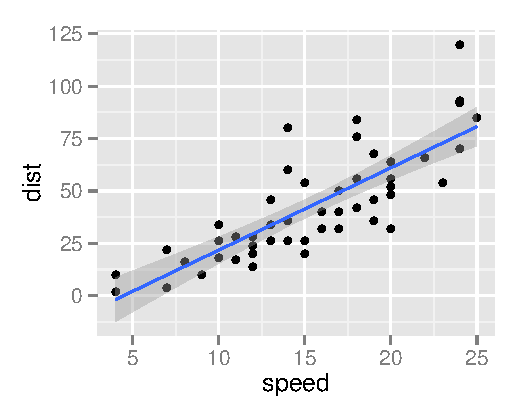
\includegraphics[width=\maxwidth]{figure/cars_plot} 

}



\end{knitrout}

\end{frame}

%}}}

\section{Design}
%{{{
\begin{frame}[fragile]
  \frametitle{How does knitr work?}
  \begin{itemize}
    \item One input file with an analysis language (R, Python, awk, SAS, \ldots)
      and an output markup language (\LaTeX, html, Markdown, \ldots)

    \item {\tt knitr} determines the appropriate set of patterns (regular
      expression to extract analysis language and options from the input file)

    \item The input file is knitted\ldots, input language is evaluated and the
      appropriate output markup results are placed into a .tex, .html, .md,
      \ldots, file.

    \item Final document (the .tex, .html, .md, \ldots)  is ready for release or
      post processing as needed.

  \end{itemize}
\end{frame} 

%}}}

\section{Options}
%{{{
\subsection{Chunk Options}
\begin{frame}[fragile]
  \frametitle{Customizing the behavior of {\tt knitr}}
  For Rnw files:

  \begin{verbatim}<<"chunk_label", echo = FALSE, results = "asis">>=
@
  \end{verbatim}
  \begin{itemize}
    \item Chunk options must be a single line, no line breaks.  
    \item Options must be valid R expressions.
    \item Chunk options can be specified for each individual chunk.
    \item Global options are set via \verb;opts_chunk$set();
  \end{itemize}
\end{frame}

\begin{frame}
  \frametitle{Chunk Options}
  Full details for all the chunk options see
  \url{http://yihui.name/knitr/options}
  \begin{itemize}
    \item Code Evaluation
    \item Text Results
    \item Code Decoration
    \item Cache
    \item Plots
    \item Animation
    \item Chunk References
    \item Child Documents
    \item Language Engines
    \item Extracting source code
  \end{itemize}
\end{frame}

\subsection{Language Options}
\begin{frame}
  \frametitle{Input/Analysis Language}
  \begin{itemize}
    \item R is the `default' language for analysis 
    \item Other options are available, including SAS.  The chunk option `engine'

      \begin{quote}
        engine: ('R'; character) the language name of the code chunk; currently
        other possible values are 'python' and 'awk'/'gawk'; the object
        knit\_engines in this package can be used to set up engines for other
        languages\footnote{http://yihui.name/knitr/options}
      \end{quote}

    \item Pick the right language for the job.  
  \end{itemize}
\end{frame}

\begin{frame}
  \frametitle{Markup Language}
  \framesubtitle{html}
  \begin{itemize}
    \item Pros: 
      \begin{itemize}
        \item easy to send to others, 
        \item comments in html, 
        \item great for tutorials or anything that will be published on line.
      \end{itemize}
    \item Cons: 
      \begin{itemize}
        \item Clunky (in my opinion), 
        \item not apt for large data analysis reports.
      \end{itemize}

    \item html code can be placed natively in markdown, ergo, markdown has
      supplants html.
  \end{itemize}
\end{frame}

\begin{frame}
  \frametitle{Markup Language}
  \framesubtitle{Markdown}
  \begin{itemize}
    \item Pros: 
      \begin{itemize}
        \item Easy to learn 
        \item Simple and versatile
        \item growing user community  
        \item Via pandoc, easy to convert to many other file formats such as
          \LaTeX\, html, or .docx.
      \end{itemize}
    \item Cons: 
      \begin{itemize}
        \item no native comments.  
        \item `too minimal'
      \end{itemize}
  \end{itemize}
\end{frame}

\begin{frame}
  \frametitle{Markup Language}
  \framesubtitle{\LaTeX}
  \begin{itemize}
    \item Pros: 
      \begin{itemize}
        \item Intended use: technical report writing and typesetting.
        \item Comments.
        \item Many tools exist for formating R output well in \LaTeX\ files.
        \item Cross referencing, citations.
      \end{itemize}

    \item Cons:
      \begin{itemize}
        \item Not so good when working with others using Microsoft Office.
        \item R is small,  Tex Live, MacTeX, and proTeXt are not.
        \item Steepest learning curve
      \end{itemize}

    \item \LaTeX\ is my preferred markup language for data analysis reports and
      presentations (via beamer).

    \item Markdown is my preferred markup language for developing a web page.
      Easier to work in than html and more flexible.

  \end{itemize} 
\end{frame}

%}}}

\section{Editors} 
%{{{
\begin{frame}
  \frametitle{Suggested Development Environments}

  \begin{itemize}
    \item For nearly all current, and new,  R programmers, 
      RStudio is the \emph{premier} R IDE.
      \begin{itemize}
        \item Download and info: \url{www.rstudio.com}

        \item Built in tools for version control, projects, knitting\ldots
      \end{itemize}

    \item I prefer the vim editor and with the vim-r-plugin.  
      \begin{itemize}
        \item Vim Editor: \url{www.vim.org/index.php}
        \item vim-r-plugin: \url{www.vim.org/scripts/script.php?script\_id=2628} 
      \end{itemize}

    \item RStudio is the better R development environment.  Vim is a better text
      editor.

    \item A pseudo WYSIWYG editor for \LaTeX\ which will work well with 
      {\tt kntir} is LyX.
      
  \end{itemize}
\end{frame}
%}}}

\section{Examples}
%{{{
\begin{frame}
  \frametitle{Reproducible examples}
  These slides, and the following examples, can be downloaded/cloned, from
  \url{https://github.com/dewittpe/knitrexamples}

  \begin{itemize}
    \item A simple data analysis report using R, and three different markup
      languages, \LaTeX, html, and Markdown.
    \item An example of using SAS within knitr.
    \item An example of a more complex and extensive data analysis report.
  \end{itemize}
\end{frame}
%}}}


%%%%%%%%%%%%%%%%%%%%%%%%%%%%%%%%%%%%%%%%%%%%%%%%%%%%%%%%%%%%%%%%%%%%%%%%%%%%%%%

\end{document} 
%%%%%%%%%%%%%%%%%%%
%%% End of File %%%
%%%%%%%%%%%%%%%%%%%

